\documentclass[../../main.tex]{subfiles}
\begin{document}

% TODO: ALL TEXT IN THIS SECTION IS WIP
Given the background and threat model detailed above, we may now
discuss the design of our system. As previously mentioned in
Section~\ref{sec:ssloverview}, the long-term private key is only
required for the SSL/TLS handshake routine. For our design, we adopt
PoLP in a manner similar to Wedge, placing the long-term private key
in an SGX enclave, and defining an interface to the private key. The
interface is designed to allow an SSL/TLS handshake to complete
successfully, without compromising the long-term private key. The
resulting, high level system architecture is depicted in
Figure~\ref{fig:sysarch}.x

\begin{figure}[H]
  \centering
  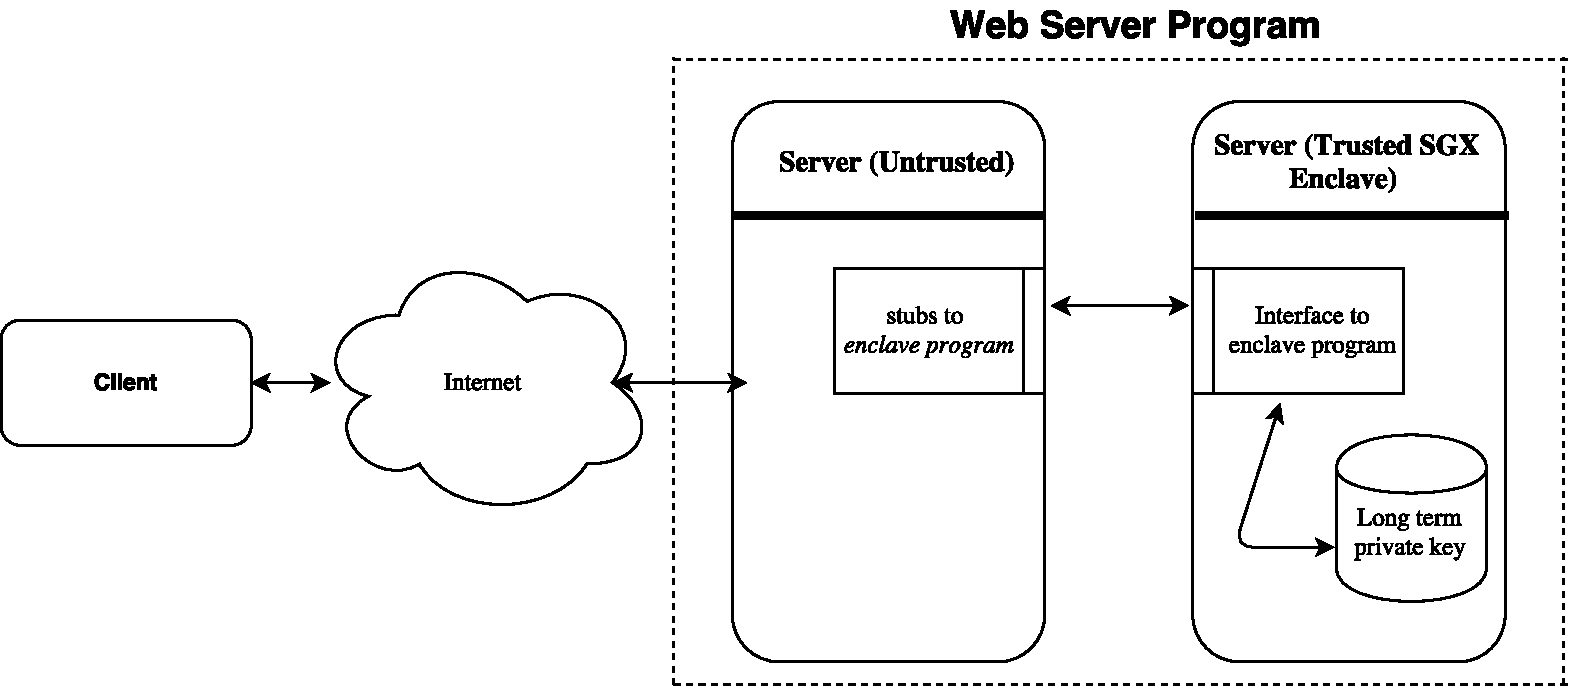
\includegraphics[scale=0.4]{images/high-level-arch.pdf}
  \caption{High Level System Architecture}
  \label{fig:sysarch}
\end{figure}

We assume that we have already invoked the above-detailed
remote-attestation mechanism to provision the enclave with the
long-term private key. The remainder of this section details the
interface design for: (1) Ciphers that do not offer forward secrecy
(2) Ciphers that offer forward secrecy.

%None of our designs modify the SSL handshake itself, though we carefully
%compartmentalize the protocol's execution in trusted and untrusted
%components. The interface for both kind of ciphers is split into two
%versions, one where only the private key of the server is protected
%and one where both the private and the session keys are protected by
%the enclave.

\end{document}
%%% Local Variables:
%%% mode: latex
%%% TeX-master: "../../main"
%%% End:
